%
%  Vincent Yannello
%
\documentclass[12pt,fullpage]{article}
\usepackage{fullpage}
\usepackage{amsmath}
\DeclareMathOperator{\erf}{erf}
\usepackage{psfrag}                                          % LaTeX graphics tool
\usepackage{pslatex}                                         % avoids the default cmr font
\usepackage{graphicx}                                        % graphics package 
\usepackage{epsfig}                                          % figures
\usepackage{epsfig} 
\usepackage{hyperref}
\usepackage{color}

\begin{document}

\noindent
{\bf Log-gamma distribution} (from \color{blue}\url{http://www.math.wm.edu/~leemis/chart/UDR/UDR.html}\color{black})

\noindent
The shorthand $X \sim$ log-gamma$(\alpha, \beta)$ is used to indicate that the
random variable $X$ has the log-gamma distribution with positive scale parameter $\alpha$ and positive shape parameter $\beta$.
A log-gamma random variable $X$ with parameters $\alpha$ and $\beta$ has probability density function 
$$
f(x) = \frac{e ^ {\kern 0.08 em \beta \kern 0.08 em x} e ^ {-e ^ {\kern 0.08 em x}/\alpha}} {\alpha ^ {\kern 0.08 em \beta}\Gamma(\beta)}
 \qquad \qquad -\infty < x < \infty.
$$
The probability density function with three different parameter combinations is illustrated below.
{\begin{figure}[h!]
\begin{center}
\psfrag{lab1}{$\alpha \kern -0.08 em = \kern -0.08 em  1,\, \beta \kern -0.08 em  = \kern -0.08 em  1$}
\psfrag{lab2}{$\alpha \kern -0.08 em  = \kern -0.08 em  5,\, \beta \kern -0.08 em  = \kern -0.08 em  1$}
\psfrag{lab3}{$\alpha \kern -0.08 em  = \kern -0.08 em  1,\, \beta \kern -0.08 em  = \kern -0.08 em  2$}
\psfrag{labx}{$x$}
\psfrag{labf}{$f(x)$}
\includegraphics[width=3.2in]{LoggammaPlot.ps}
\end{center}
\end{figure}}\\
The cumulative distribution, survivor function, hazard function, cumulative hazard 
function, inverse distribution function, moment generating function, and characteristic function
on the support of $X$ are mathematically intractable. The population mean, variance, skewness, and kurtosis of $X$ are also mathematically intractable.

\vspace{0.1in}

\noindent
{\bf APPL failure:}
The APPL statements
\begin{verbatim}
X := [[exp(beta * x) * exp(-exp(x) / alpha) / (alpha ^ beta * GAMMA(beta))],
      [-infinity,infinity],["Continuous", "PDF"]];
Mean(X);
Variance(X);
Skewness(X);
Kurtosis(X);
MGF(X);
\end{verbatim}
fails to return the population mean, variance, skewness, kurtosis, and moment generating function.

\end{document}
